% !TEX TS-program = lualatex
%\documentclass[handout]{beamer}
\documentclass{beamer}
\input{../common/misomva}
\newcommand{\misoclasstinytitleslide}{Partially based on material by:  Ulrike von Luxburg, \\[-1em] Gary Miller, Doyle \& Schnell, Daniel Spielman}
\newcommand{\misoclassdate}{}
\usetikzlibrary{graphs}

\begin{document}
% Topic-specific title slide

\newcommand{\topictitle}{Graph Laplacian Basics}

\newcommand{\topicsubtitle}{Definition, Properties, Smoothness}

\MakeTopicSlide

\begin{frame}
\frametitle{Graph Laplacian}
\begin{center}
$\cG = (\nodeset, \edgeset)$ - with a set of \textbf{nodes} $\nodeset$ and a set of \textbf{edges} $\edgeset$    \\\bigskip \pause
\begin{tabular}{cl}
$\bA$  &  adjacency matrix \\ \pause
$\bW$ & weight matrix  \\ \pause
$\bD$  & (diagonal) degree matrix \\ \pause
$\bL = \bD - \bW$  & graph \gcol{Laplacian} matrix 
\end{tabular}

\begin{columns}[c]
\column{1.4in}
{\scriptsize
\null\smallskip\specialcell{
\begin{math}
\bL = \left(
\begin{array}{rrrrr}
4 & -1 & 0 & -1 & -2 \\
-1 & 8 & -3 & -4 & 0 \\
0 & -3 & 5 & -2 & 0 \\
-1 & -4 & -2 & 12 & -5 \\
-2 & 0 & 0 & -5 & 7 \\
\end{array}
\right)
\end{math}
}
}
\vskip 1cm
\yellbox{$\bL$ is SDD!}
\column{2.5in}
\begin{center}
%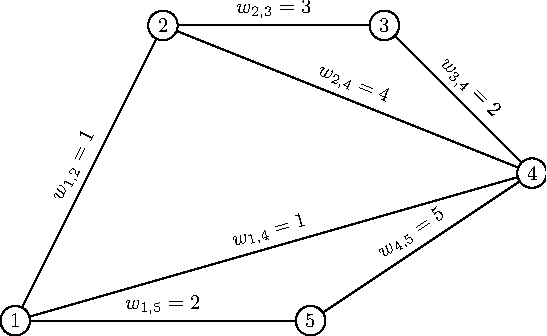
\includegraphics[width=2in]{../img/lap.pdf}
% Manual layout for weighted graph (spring layout needs lualatex)
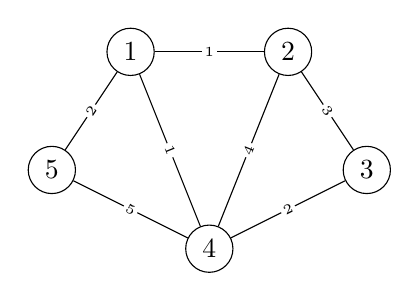
\begin{tikzpicture}[
  nd/.style={circle, draw, minimum size=6mm, inner sep=0pt},
  lbl/.style={font=\tiny, fill=white, inner sep=1pt, sloped, midway}]
\node[nd] (1) at (0,1.5) {1};
\node[nd] (2) at (2,1.5) {2};
\node[nd] (3) at (3,0) {3};
\node[nd] (4) at (1,-1) {4};
\node[nd] (5) at (-1,0) {5};
\draw (1) -- node[lbl] {1} (2);
\draw (2) -- node[lbl] {3} (3);
\draw (3) -- node[lbl] {2} (4);
\draw (4) -- node[lbl] {1} (1);
\draw (1) -- node[lbl] {2} (5);
\draw (5) -- node[lbl] {5} (4);
\draw (4) -- node[lbl] {4} (2);
\end{tikzpicture}

\end{center}

\end{columns}
\phantom{a}\\[0.05em]
{\tiny demo: \url{https://dominikschmidt.xyz/spectral-clustering-exp/}}\\

\end{center}
\end{frame}




%%%%%%%%%%%%%%%%%%%%%%%%%%%%%%%%%%%%%%%%%%%%%%%%%%%%%%%%%%%%%
\begin{frame}
\frametitle{Properties of Graph Laplacian}

\begin{block}{}
\gcol{Graph function}: a vector $\bff \in \R^\nodes$ assigning values to nodes: $$\bff : \nodeset(\cG) \to \R.$$
\end{block}

\pause

\begin{block}{}
$$\bff\transpose\bL\bff = \frac{1}{2}\sum_{i,j\leq \nodes}w_{i,j}(f_i-f_j)^2 \pause= S_G(\bff)$$
\end{block}

\pause
\onslide<handout:0>{\notecol{%
\textbf{Proof:}
{\footnotesize
\begin{align*}
\bff\transpose\bL\bff &= \sum_{i,j \leq \nodes} \bL_{i,j}f_if_j = \sum_{i,j \leq \nodes} \bD_{i,j}f_if_j - \sum_{i,j \leq \nodes} \bW_{i,j}f_if_j = \sum_{i=1}^\nodes d_if_i^2-\sum_{i,j\leq \nodes}w_{i,j}f_if_j \\
&= \frac{1}{2}\left( \sum_{i=1}^\nodes d_if_i^2 - 2\sum_{i,j\leq \nodes}w_{i,j}f_if_j + \sum_{j=1}^\nodes  d_if_j^2\right) = \frac{1}{2}\sum_{i,j\leq \nodes} w_{i,j}(f_i-f_j)^2
%&= \frac{1}{2}\left( \sum_{i=1}^\nodes d_if_i^2 - 2\sum_{i,j\leq \nodes}w_{i,j}f_if_j + \sum_{j=1}^\nodes  d_if_j^2\right) = \frac{1}{2}\sum_{i,j\leq \nodes} w_{i,j}(f_i-f_j)^2
\end{align*}
}}}

\end{frame}
%%%%%%%%%%%%%%%%%%%%%%%%%%%%%%%%%%%%%%%%%%%%%%%%%%%%%%%%%%%%%
\begin{frame}
\frametitle{Review: Eigenvalues and Eigenvectors}

A vector $\bv$ is an \gcol{eigenvector} of matrix $\bM$ of \gcol{eigenvalue}
$\lambda$ 
\vspace{-0.1cm}
$$\bM\bv = \lambda\bv.$$ 
\vspace{-0.8cm}
\pause

\begin{block}{}
If $(\lambda_1,\bv_1)$ are $(\lambda_2,\bv_2)$ \gcol{eigenpairs}
for symmetric $\bM$  with $\lambda_1 \ne \lambda_2$ then 
$\bv_1 \perp \bv_2$, i.e., $\bv_1\transpose \bv_2 = 0$. \\
\end{block}
\pause
\onslide<handout:0>{\notecol{%
 Proof: $\lambda_1 \bv_1\transpose \bv_2 
= \bv_1\transpose \bM \bv_2 
= \bv_1\transpose \lambda_2 \bv_2
= \lambda_2 \bv_1\transpose \bv_2 \implies \bv_1\transpose \bv_2 = 0$}} 
\pause
\begin{block}{}
If $(\lambda,\bv_1)$, $(\lambda,\bv_2)$ are eigenpairs
for $\bM$ then $(\lambda,\bv_1 + \bv_2)$ is as well.\\
\end{block}
\pause
\begin{block}{}
For symmetric $\bM$, the \gcol{multiplicity} of $\lambda$ is the dimension of the 
space of eigenvectors corresponding to $\lambda$.
\end{block}

\begin{block}{}
$\nodes \times \nodes$ symmetric matrix has $\nodes$ eigenvalues (w/ multiplicities).
\end{block}

\end{frame}


%%%%%%%%%%%%%%%%%%%%%%%%%%%%%%%%%%%%%%%%%%%%%%%%%%%%%%%%%%%%%
\begin{frame}
\frametitle{Eigenvalues, Eigenvectors, and Eigendecomposition}

\tikzstyle{every picture}+=[remember picture]
% \tikzstyle{na} = [baseline=-.5ex]

\notecol{
A vector $\bv$ is an \textbf{eigenvector} of matrix $\bM$ of \textbf{eigenvalue} 
$\lambda$ $$\bM\bv = \lambda\bv.$$ }
\vspace{-0.5cm}


Vectors $\{\bv_i\}_i$ form an \textbf{orthonormal} basis with 
$ \lambda_1 \leq \lambda_2 \leq \dots \lambda_\nodes$.

$$ \forall i \quad \bM\bv_i = \lambda_i\bv_i \pause 
\qquad \equiv \qquad 
\tikz[baseline]{\node[anchor=base, onslide=<3->{fill=mvaHighlight}] (a1) {$\bM\bQ = \bQ\bLambda$};}
$$ 
\notecol{\small $\bQ$ has eigenvectors in columns and $\bLambda$ has eigenvalues on its diagonal.}
 \pause
\begin{block}{}
Right-multiplying $\bM\bQ = \bQ\bLambda$ by $\bQ\transpose$ we get the \gcol{eigendecomposition} of $\bM$: 
\vspace{-0.2cm}
$$
 \bM = 
\tikz[baseline]{\node[anchor=base, onslide=<3->{fill=mvaHighlight}] (b1) {$\bM \bQ \bQ\transpose  = \bQ\bLambda\bQ\transpose $};}
= \textstyle\sum_i\lambda_i\bv_i\bv_i\transpose
$$
\vspace{-0.6cm}
\end{block}

% \pause
\begin{tikzpicture}[overlay]
\path<3->[->,line width=1.5pt,draw=mvaHighlight] (a1) edge [bend left=44] (b1);
\end{tikzpicture}

\end{frame}

%%%%%%%%
\begin{frame}
\frametitle{$\bM = \bL$: Properties of Graph Laplacian}

We can assume \textbf{non-negative weights}: $w_{ij} \geq 0$.
\pause
\begin{block}{}
$\bL$ is symmetric
\end{block}
\pause
\begin{block}{}
$\bL$ positive semi-definite \pause $\gets \bff\transpose\bL\bff = \frac{1}{2}\sum_{i,j\leq \nodes}w_{i,j}(f_i-f_j)^2$
\end{block}
\pause
Recall: If $\bL \bff = \lambda \bff$ then $\lambda$ is an \textbf{eigenvalue} (of the Laplacian).
\pause
\begin{block}{}
The smallest eigenvalue of $\bL$ is 0. Corresponding eigenvector: $\bOne_\nodes$.
\end{block}
\pause
\begin{block}{}
All eigenvalues are non-negative reals $0 = \lambda_1 \leq \lambda_2 \leq \dots \leq \lambda_\nodes$. 
\end{block}
\pause
\begin{block}{}
Self-edges do not change the value of $\bL$. 
\end{block}

\end{frame}
%%%%%%%%%%%%%%%%%%%%%%%%%%%%%%%%%%%%%%%%%%%%%%%%%%%%%%%%%%%%%

\begin{frame}
\frametitle{Properties of Graph Laplacian}

\begin{block}{}
The multiplicity of eigenvalue 0 of $\bL$ equals to the number of connected components.
The eigenspace of 0 is spanned by the components' indicators.
\end{block}
\pause
Proof: If $(0,\bff)$ is an eigenpair then $0 = \frac{1}{2}\sum_{i,j\leq \nodes}w_{i,j}(f_i-f_j)^2$.
\pause
Therefore, $\bff$ is constant on each connected component.
\pause
If there are~$k$ components, then $\bL$ is $k$-block-diagonal:
$$
 \bL = 
\left[\begin{array}{cccc}
\bL_{1}& &  &\\
&\bL_{2}& & \\
& &\ddots & \\
& & &\bL_{k}\\
\end{array}\right]
$$
\pause
For block-diagonal matrices: the spectrum is the union of the spectra of $\bL_i$
\pause
(eigenvectors of $\bL_i$ padded with zeros elsewhere).
\pause
\begin{flushright}
For $\bL_i$ $(0,\bOne_{|V_i|})$ is an eigenpair, hence the claim.
\end{flushright}
\end{frame}
%%%%%%%%%%%%%%%%%%%%%%%%%%%%%%%%%%%%%%%%%%%%%%%%%%%%%%%%%%%%%








\MakeLastSlide
\end{document}
